\chapter{System Design}
\section{System Architecture}
The React frontend calls FastAPI routes. The shared service orchestrator freezes the candidate, routes applicable analyzers, stores their evidence and events, and asks the shared final gate to validate current bindings and compute the workflow result. Module-specific interfaces remain available in addition to the shared Run Workflow. Figure~\ref{fig:asent-overall-architecture} is page 02 of the editable diagrams.net source \texttt{ASENT\_All\_Diagrams.drawio}; its labels and flow correspond to the current local application.

\begin{landscape}
\begin{figure}[p]
\centering
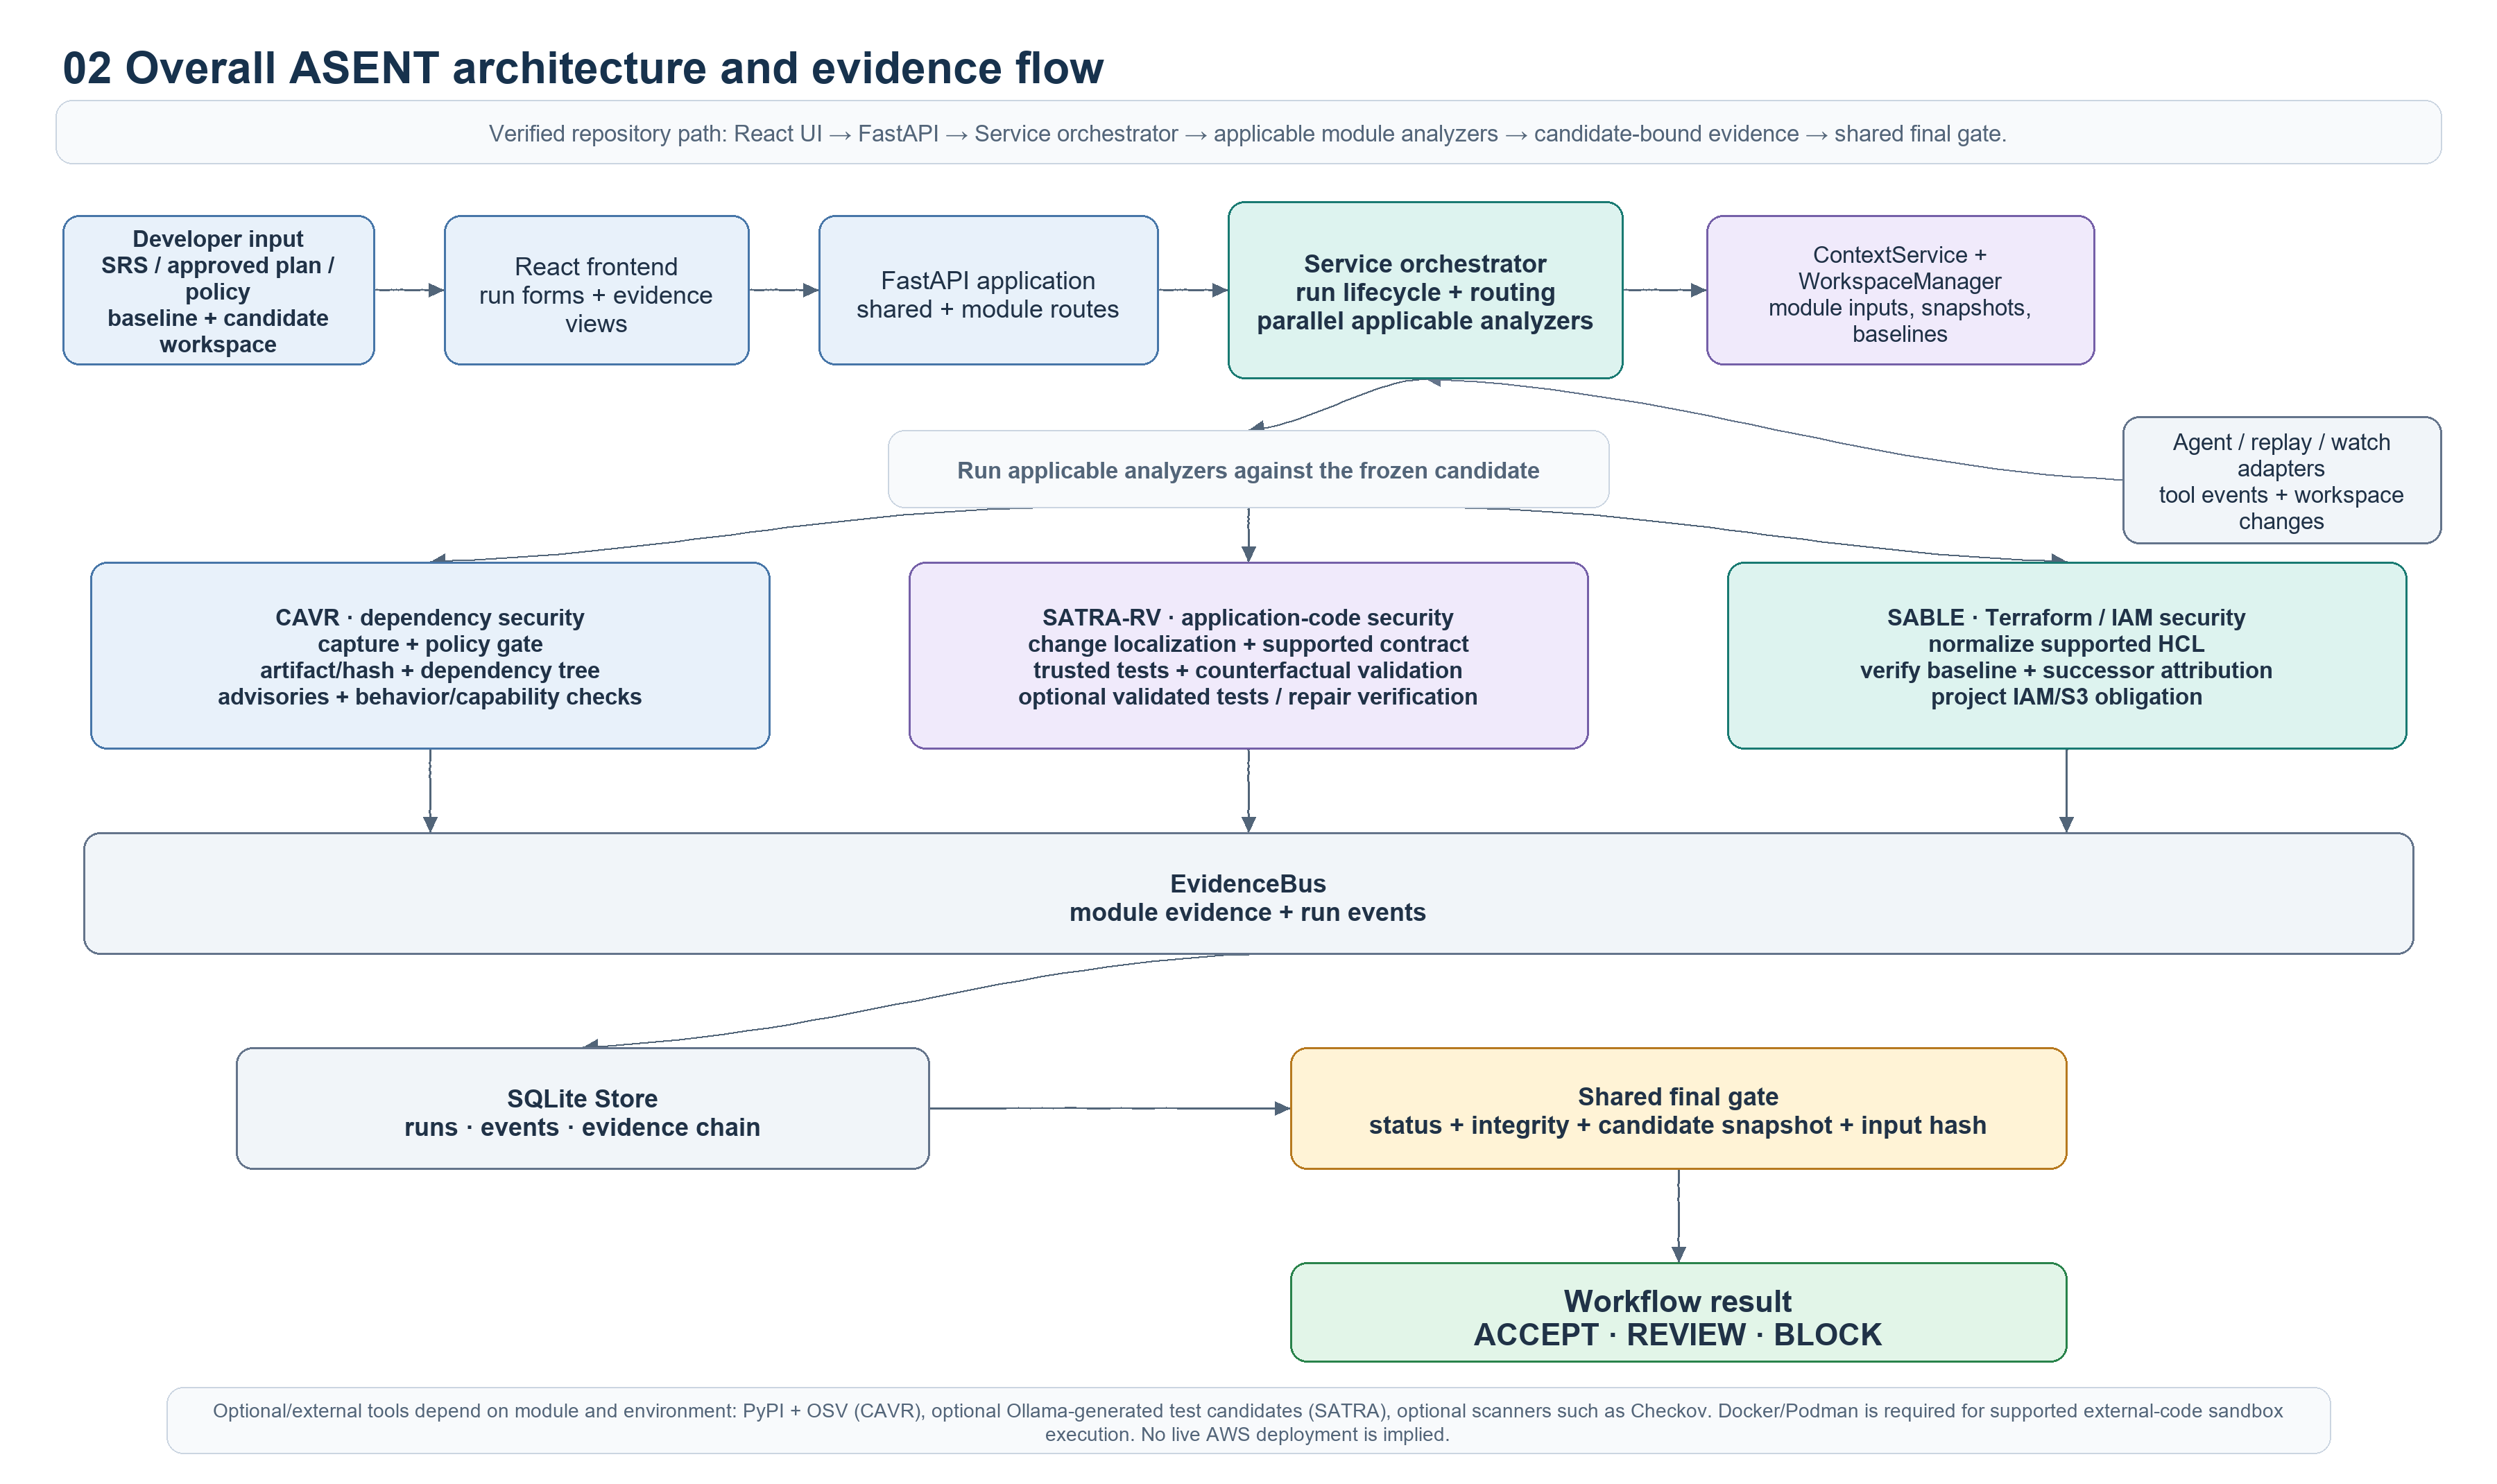
\includegraphics[width=0.97\linewidth,height=0.84\textheight,keepaspectratio]{figures/asent/asent-architecture.png}
\caption{Implemented ASENT architecture and evidence flow. Applicable analyzers publish module evidence through the local evidence bus/store; the shared final gate checks evidence bindings before returning an overall result. This is not a hosted deployment diagram.}
\label{fig:asent-overall-architecture}
\end{figure}
\end{landscape}

\section{Process and Shared Decision Design}
The SABLE behavior in Figure~\ref{fig:sable-current-process} is page 07 of the editable diagrams.net source. Its decision order is grounded in \path{backend/sable/analyzer.py}, \path{backend/sable/correspondence.py}, and the authorization evaluators: verify the trusted baseline obligation, rank candidate successors, and evaluate the same principal/action/resource scope against the selected successor. If the baseline, correspondence, binding, or authorization semantics are insufficient, the result remains \texttt{UNKNOWN}.

\begin{landscape}
\begin{figure}[p]
\centering
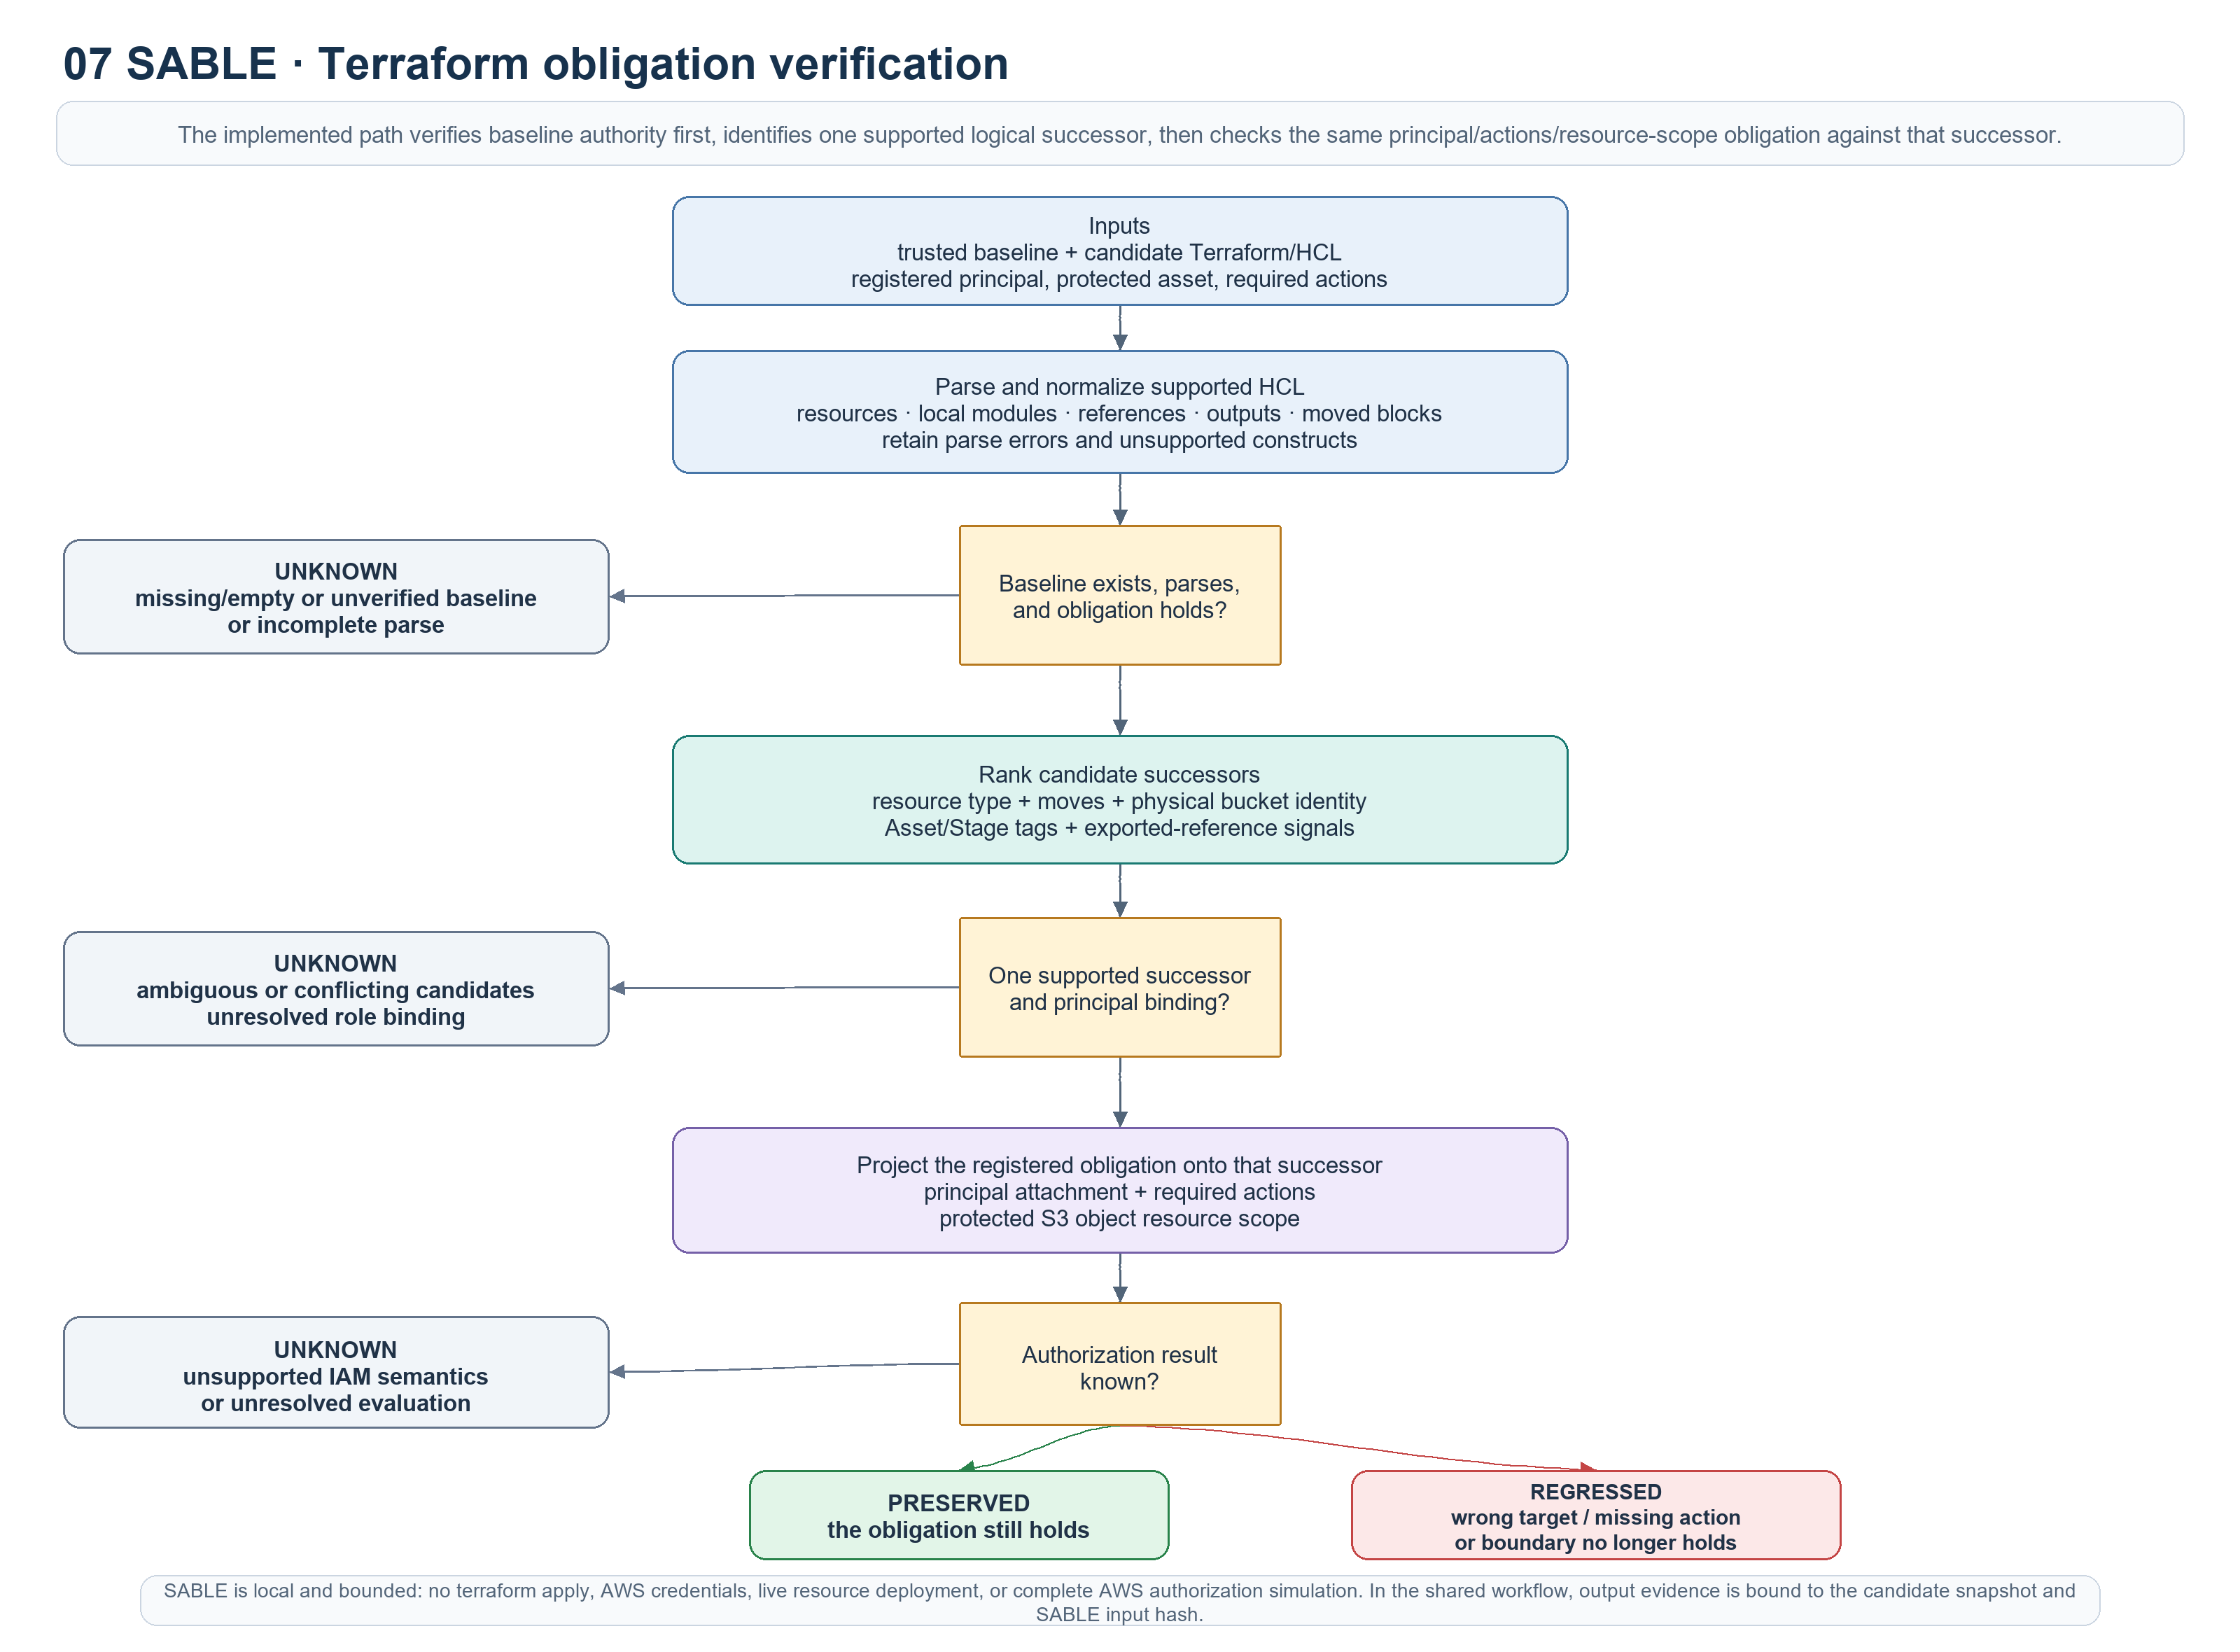
\includegraphics[width=0.97\linewidth,height=0.84\textheight,keepaspectratio]{figures/asent/sable-assurance-flow.png}
\caption{SABLE baseline-first Terraform obligation verification from page 07 of the editable diagrams.net source. No Terraform apply or live AWS authorization query is part of this path.}
\label{fig:sable-current-process}
\end{figure}
\end{landscape}

The shared final gate is a separate operation from the module verdict. Figure~\ref{fig:asent-shared-final-gate} is page 09 of the same editable source and shows how applicable CAVR, SATRA-RV, and SABLE statuses are combined only after evidence integrity, candidate snapshot, and input hashes are checked. A preserved SABLE result alone therefore does not imply an overall \texttt{ACCEPT}.

\begin{landscape}
\begin{figure}[p]
\centering
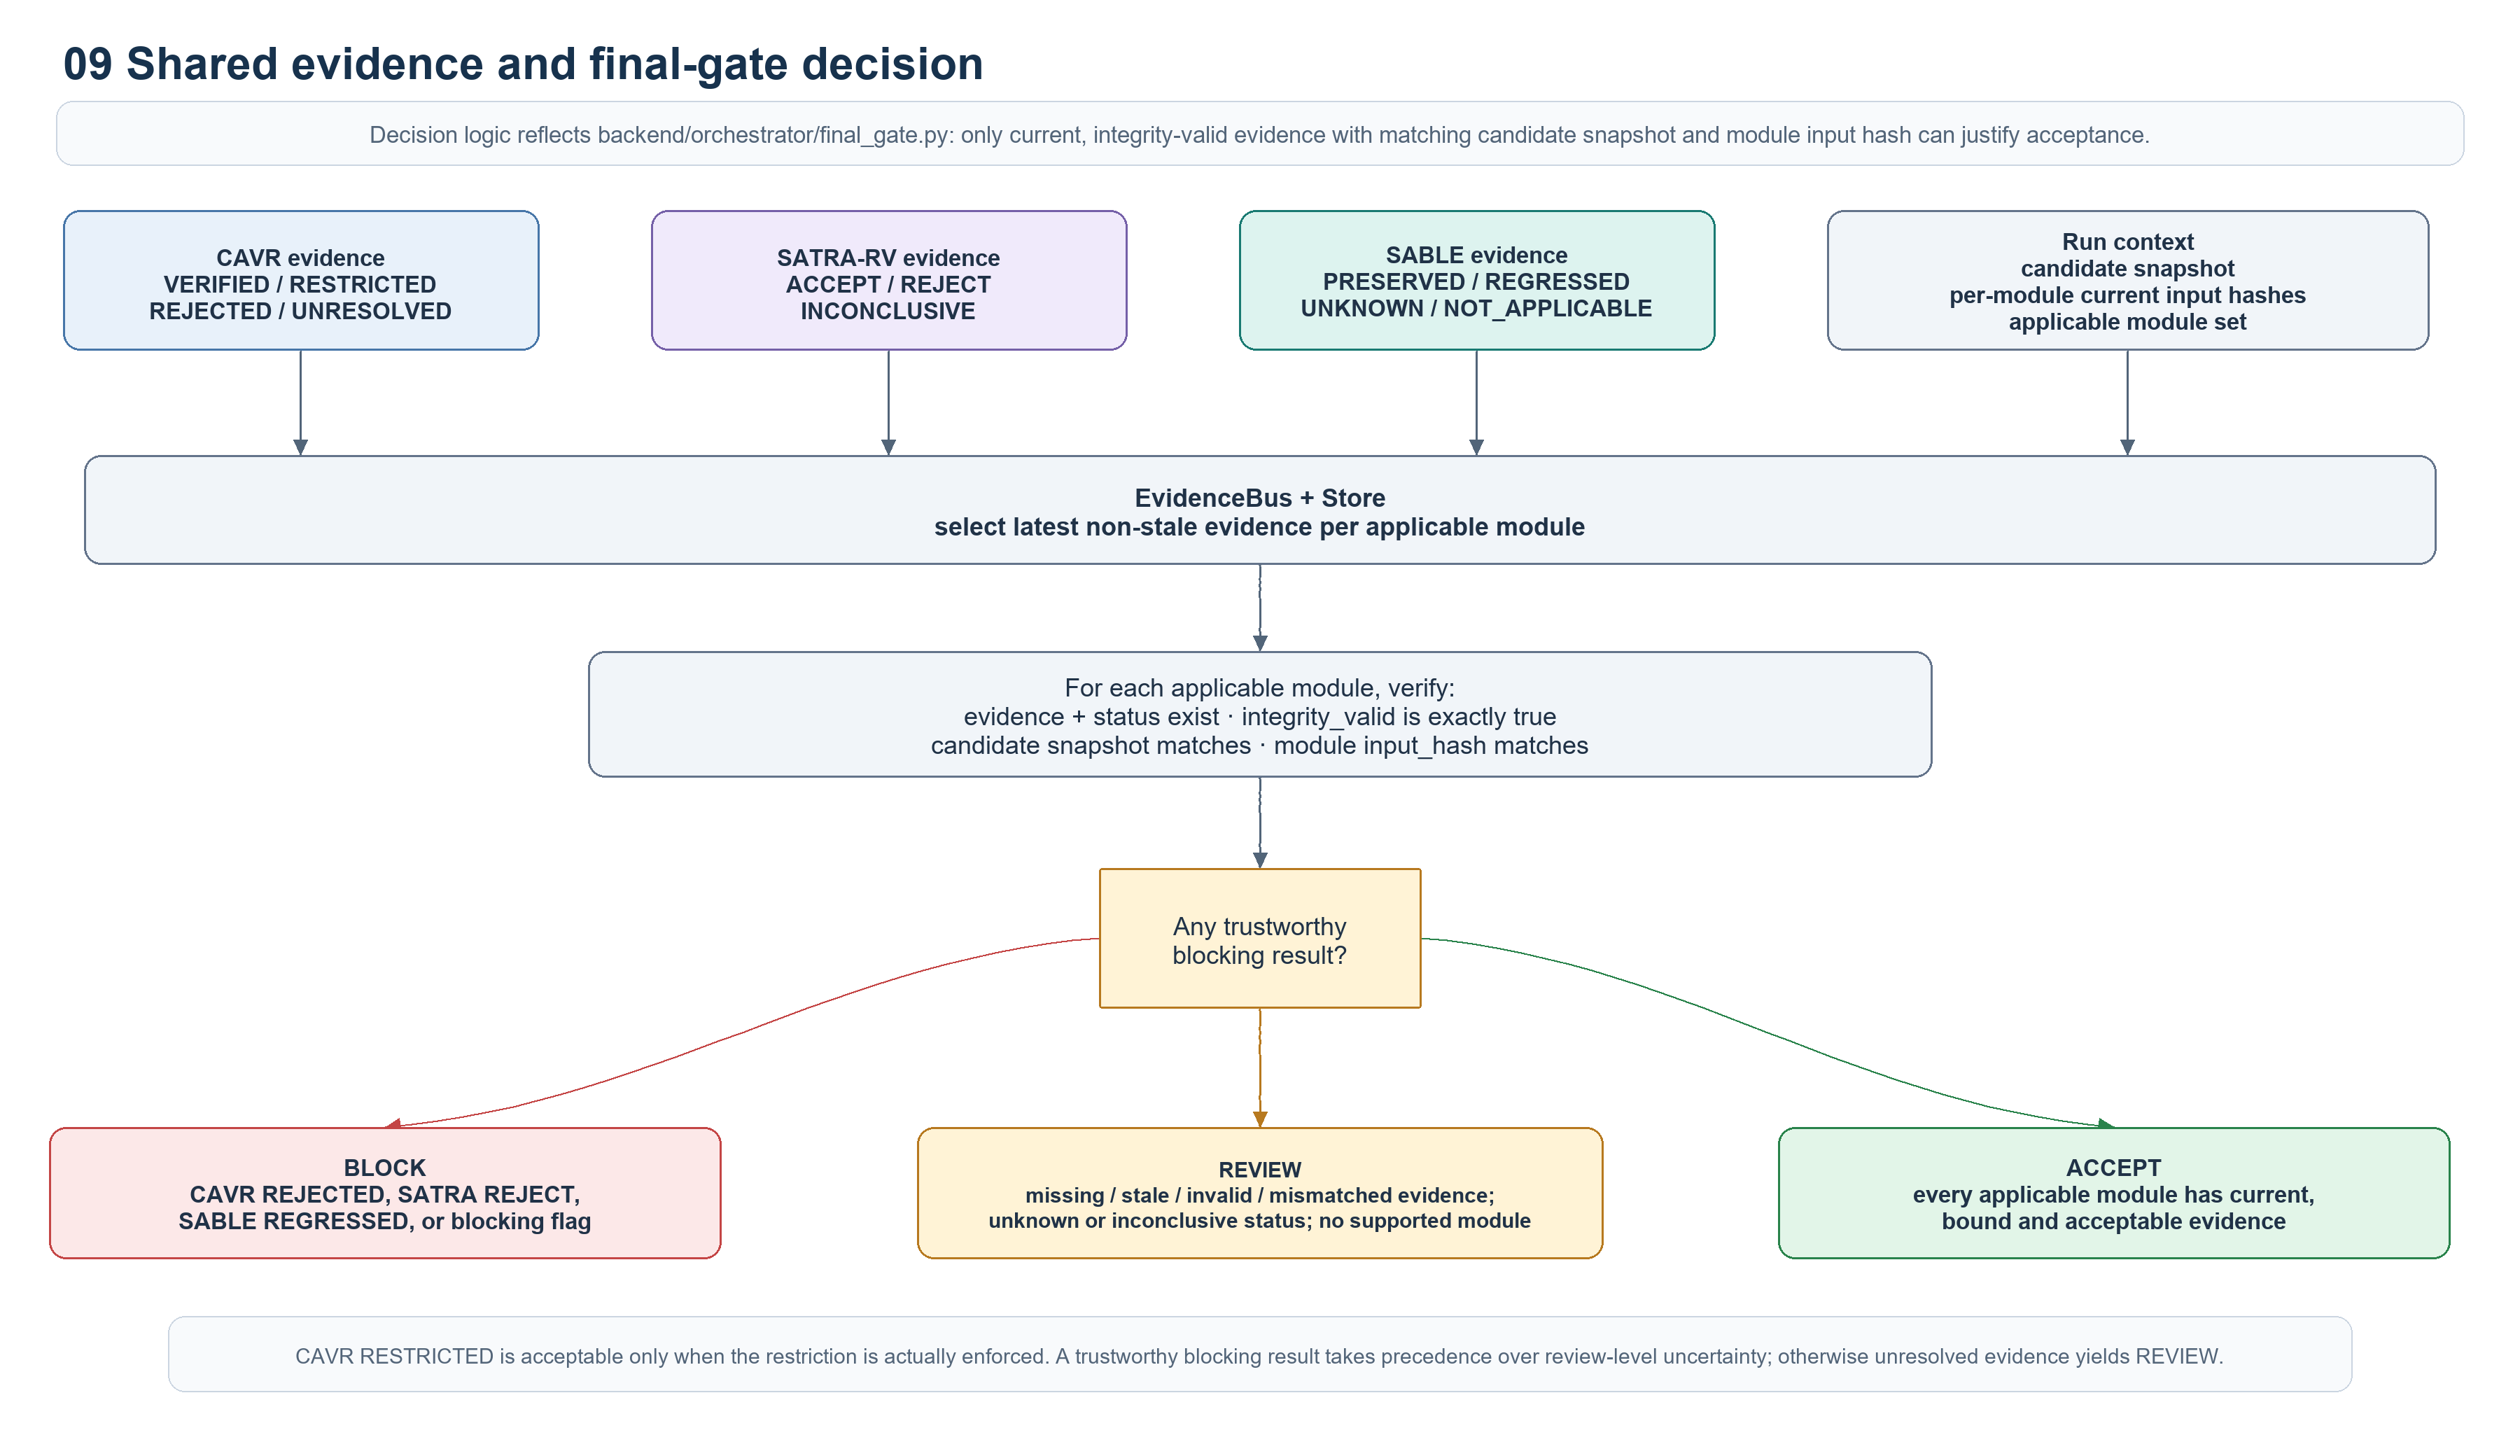
\includegraphics[width=0.97\linewidth,height=0.84\textheight,keepaspectratio]{figures/asent/shared-final-gate.png}
\caption{Shared final-gate outcomes from page 09 of the editable diagrams.net source. A trustworthy blocking status yields \texttt{BLOCK}; incomplete, stale, mismatched, invalid, or inconclusive evidence requires \texttt{REVIEW}; \texttt{ACCEPT} requires all applicable evidence to be acceptable.}
\label{fig:asent-shared-final-gate}
\end{figure}
\end{landscape}

CAVR \texttt{RESTRICTED} is accepted by the gate only when the restriction is enforced; no current CAVR path emits it.

\section{Architectural Components}
\begin{longtable}{p{0.27\textwidth}p{0.65\textwidth}}
\caption{Architectural Components -- supporting table 1}\\
\toprule
\textbf{Component} & \textbf{Implemented responsibility}\\
\midrule
\path{backend/sable/analyzer.py} & Coordinates the baseline check, candidate analysis, correspondence, authorization projection, scenario result, and evidence details.\\
\path{backend/sable/hcl_parser.py} & Parses the supported HCL input and normalizes resource records, references, local-module outputs, and moved-block data.\\
\path{backend/sable/correspondence.py} & Scores same-type candidate successors using address, move, physical bucket, tags, lifecycle, and exported-reference signals; rejects conflicting or insufficiently separated candidates.\\
\path{backend/sable/authorization.py} & Standalone SABLE evaluator for the bounded policy model, including principal attachment, actions, resource scope, denies, and unsupported/unresolved conditions.\\
\path{backend/sable/policy\_semantics.py} & Shared analysis evaluator for its supported inline role-policy subset; the regression suite compares required cases across the two evaluators.\\
\path{backend/orchestrator/service.py} & Runs applicable analyzers and publishes evidence for the shared workflow with candidate and input bindings.\\
\path{backend/orchestrator/final\_gate.py} & Validates current evidence and maps module statuses into the workflow decision; another module may independently cause review or block.\\
\bottomrule
\end{longtable}

\section{Interfaces and Dependencies}
SABLE consumes baseline and candidate workspaces plus the registered obligation through the module context and API. HCL parsing uses \texttt{python-hcl2}; the resource-reference graph uses NetworkX. The service/API layer uses FastAPI and Pydantic. In the integrated route, the orchestrator stores SABLE evidence and the final gate consumes it. This report's tested shared route is exercised by \path{test_shared_sable_evidence_drives_final_gate}; the standalone SABLE UI and API are distinct entry points.

\section{Architecture Decisions and Rationale}
The central decision is to separate authorization validity from logical-asset correspondence. A policy may allow the required actions against a bucket and still fail the registered obligation if that bucket is not the protected successor. The system therefore verifies the trusted baseline, establishes a supported successor, then checks authorization on that successor. This order directly addresses the wrong-target fixture and prevents a candidate-local allow from being treated as proof of continuity.

Uncertainty is a first-class result. The successor selector abstains on ambiguity or conflicting signals, and unsupported or unresolved policy semantics remain unknown. The shared final gate independently checks evidence freshness, input binding, and integrity. This bounded design makes the evidence path inspectable without claiming arbitrary Terraform equivalence or complete AWS semantics.

\section{Design Evolution}
The implemented design retains B0--B4 analysis configurations for the planned comparison described in the SABLE research design. This is not evidence that a comparative research experiment has been completed. A focused correctness audit found a difference between the standalone and shared authorization evaluators for unresolved role attachment: the shared path returned unknown while standalone analysis ignored a dynamic binding. The standalone evaluator now marks unresolved bindings outside its model, while retaining the behavior that a statically known unrelated role can be ignored. Tests \path{test_sable_standalone_evaluator_fails_closed_on_unresolved_role_binding} and \path{test_sable_explicitly_unrelated_role_binding_is_ignored} cover both sides. The correction was committed as \texttt{58b0a3d}. A later gate audit corrected missing/empty baselines to SABLE \texttt{UNKNOWN}, makes SABLE \texttt{NOT\_APPLICABLE} yield final \texttt{REVIEW}, and requires integrity to be explicitly true with matching candidate and module-input bindings. These corrections are covered by tests and are present in source commit \texttt{84f91a9}, which is part of the integrated PR~\#5 change. The exact tested PR head was \texttt{554b6d51}; all 18 check runs succeeded before it was merged as \texttt{ffe8aa91}. The original 44-test CI run predates the unresolved-binding and later gate corrections; Chapter 7 separates all result provenance.

\section{Domain Model}
The principal domain objects are the trusted baseline obligation (identifier, principal, protected asset, required actions and scope), normalized Terraform resources and references, successor hypotheses with evidence signals, authorization evaluation, candidate-bound module evidence, and the shared decision. The obligation under the acceptance tests is \texttt{S3-APPROLE-CUSTOMERDATA}.

The editable diagrams.net source page 08 separates the registered obligation, baseline and candidate resource models, successor hypothesis, authorization projection, module result, bound evidence, and shared final decision. Figure~\ref{fig:sable-domain-model} uses that source page directly; correspondence and authorization are shown as distinct operations because the implementation first chooses a supported successor and then checks the obligation on it.

\begin{landscape}
\begin{figure}[p]
\centering
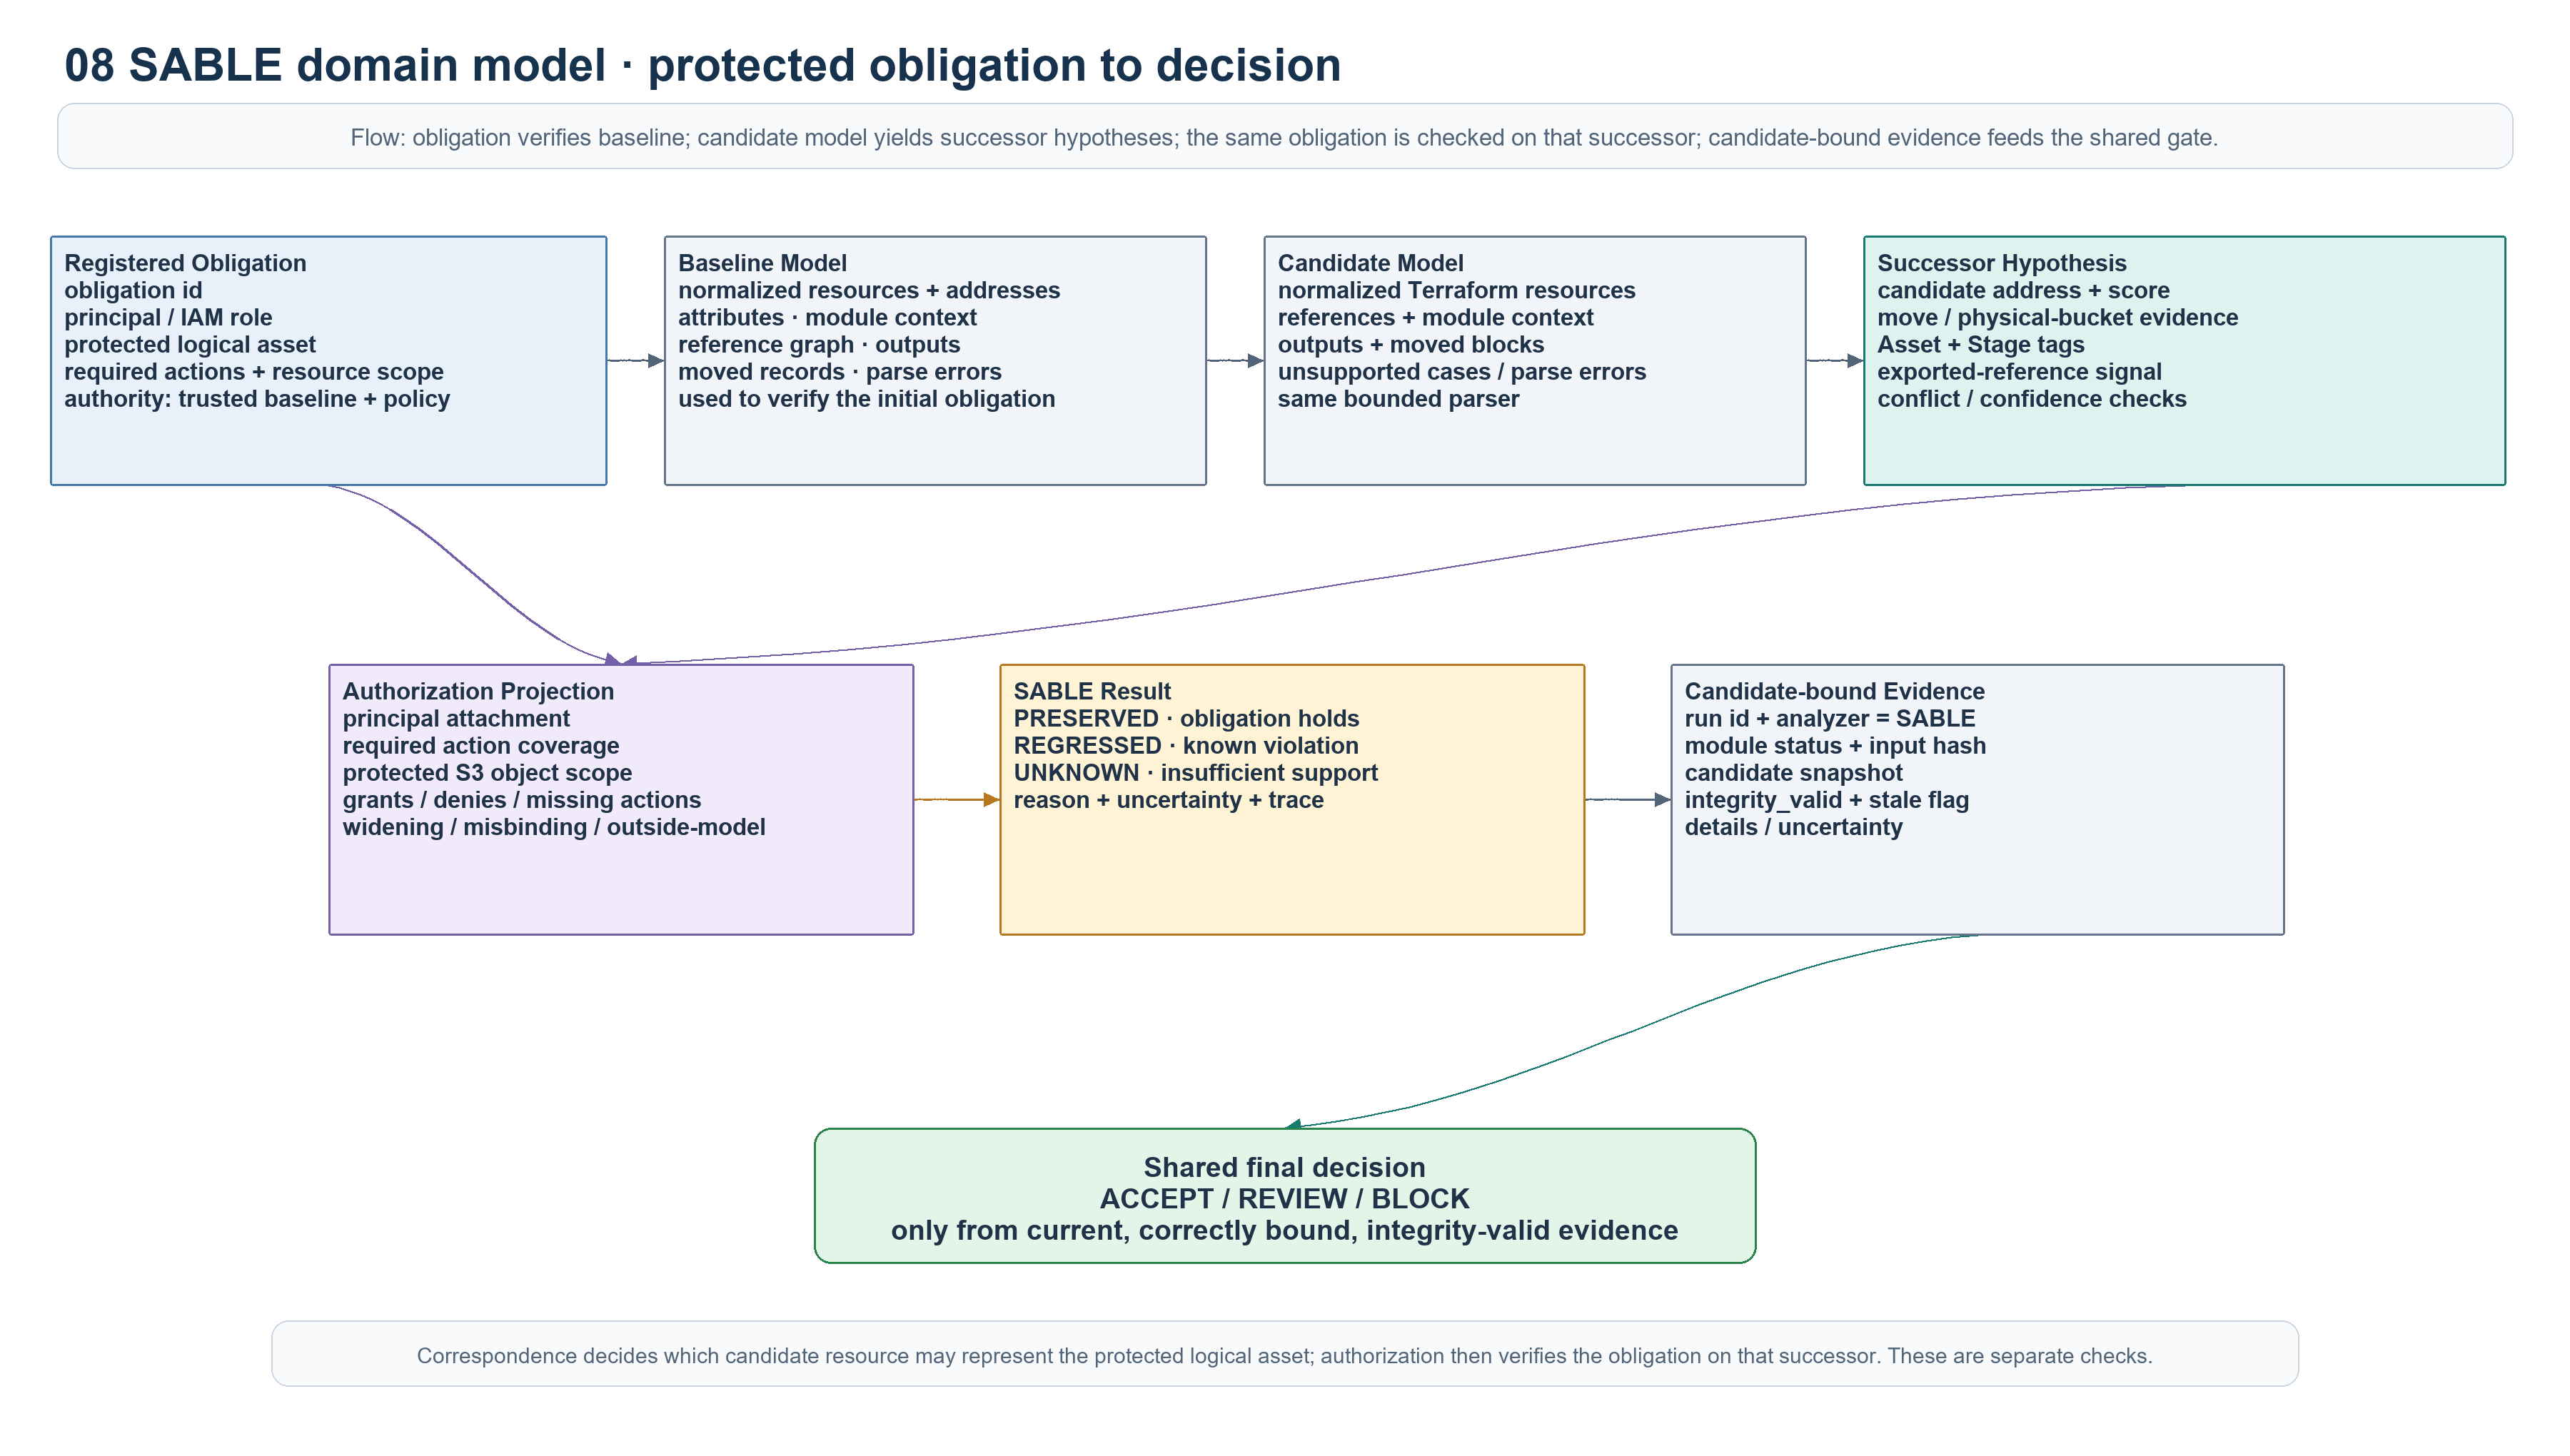
\includegraphics[width=0.97\linewidth,height=0.84\textheight,keepaspectratio]{figures/asent/sable-domain-model.png}
\caption{SABLE domain model from page 08 of the editable diagrams.net source. Evidence is eligible for the shared decision only when it is current, candidate-bound, integrity-valid, and matched to the module input.}
\label{fig:sable-domain-model}
\end{figure}
\end{landscape}

\section{Data Design}
\begin{figure}[htbp]
\centering
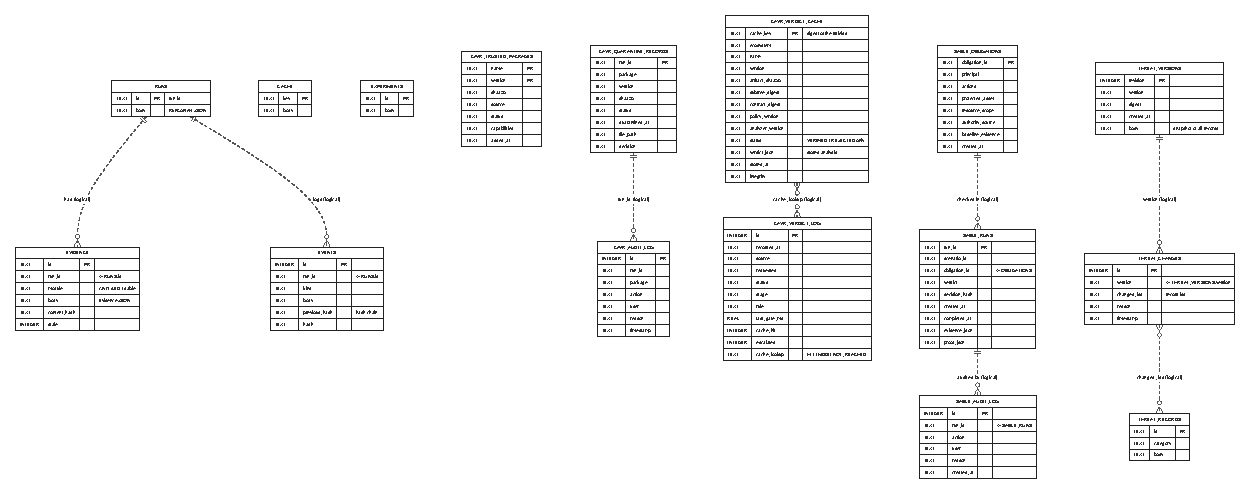
\includegraphics[width=\textwidth]{figures/diagrams/erd.pdf}
\caption{Entity--relationship diagram of the SQLite stores (\texttt{db/storage.py}, \texttt{cavr/storage.py}, \texttt{sable/storage.py}, \texttt{threat\_repo/repository.py}). Dashed relationships are logical: the code writes the same identifier into both tables but declares no foreign keys.}
\label{fig:asent-erd}
\end{figure}

Figure~\ref{fig:asent-erd} shows the persistent data. The shared run store keeps each run as a \texttt{RunContext} JSON document, the module evidence bound to it (with a content hash and a stale flag) and the run events as a hash chain. The CAVR store holds the M1 \texttt{verdict\_cache}, keyed by a digest of the eight key fields and storing only complete analyses with an integrity value, and the \texttt{verdict\_log}, one row per request, from which the cache hit rate and the p50/p95 latency are computed; the trusted-package, quarantine and audit tables come from the earlier prototype. The SABLE store holds registered obligations, SABLE runs and their audit log, and the threat repository versions its records so that every change has a version and a reason. Integrity is enforced by the code (shared identifiers, content hashes, hash chains) rather than by declared foreign keys.

The parser's normalized resource model carries Terraform address, type, attributes, module context, and graph references. Correspondence returns ranked hypotheses and conflict reasons. Authorization results contain known/holds values, expected and unexpected resources, missing actions, widening, misbinding, and outside-model evidence. The orchestrator evidence includes run identity, analyzer, candidate snapshot, input hash, status, stale state, and integrity result. The gate uses these fields to decide whether evidence is current and trustworthy.

\section{Process / Behavior Design}
The sequence in Figure~\ref{fig:sable-current-process} is fail-closed at decision boundaries: a missing, empty, or unverified baseline cannot establish continuity; no unique supported successor means no projected safe result; unsupported policy meaning cannot prove the obligation; SABLE \texttt{NOT\_APPLICABLE} and stale, mismatched, or integrity-invalid evidence cannot establish acceptance. The shared gate requires \texttt{integrity\_valid} to be exactly true and checks candidate-snapshot and module-input-hash bindings. Tests exercise these conditions and map unknown or not-applicable SABLE evidence to final \texttt{REVIEW}.

\begin{figure}[htbp]
\centering
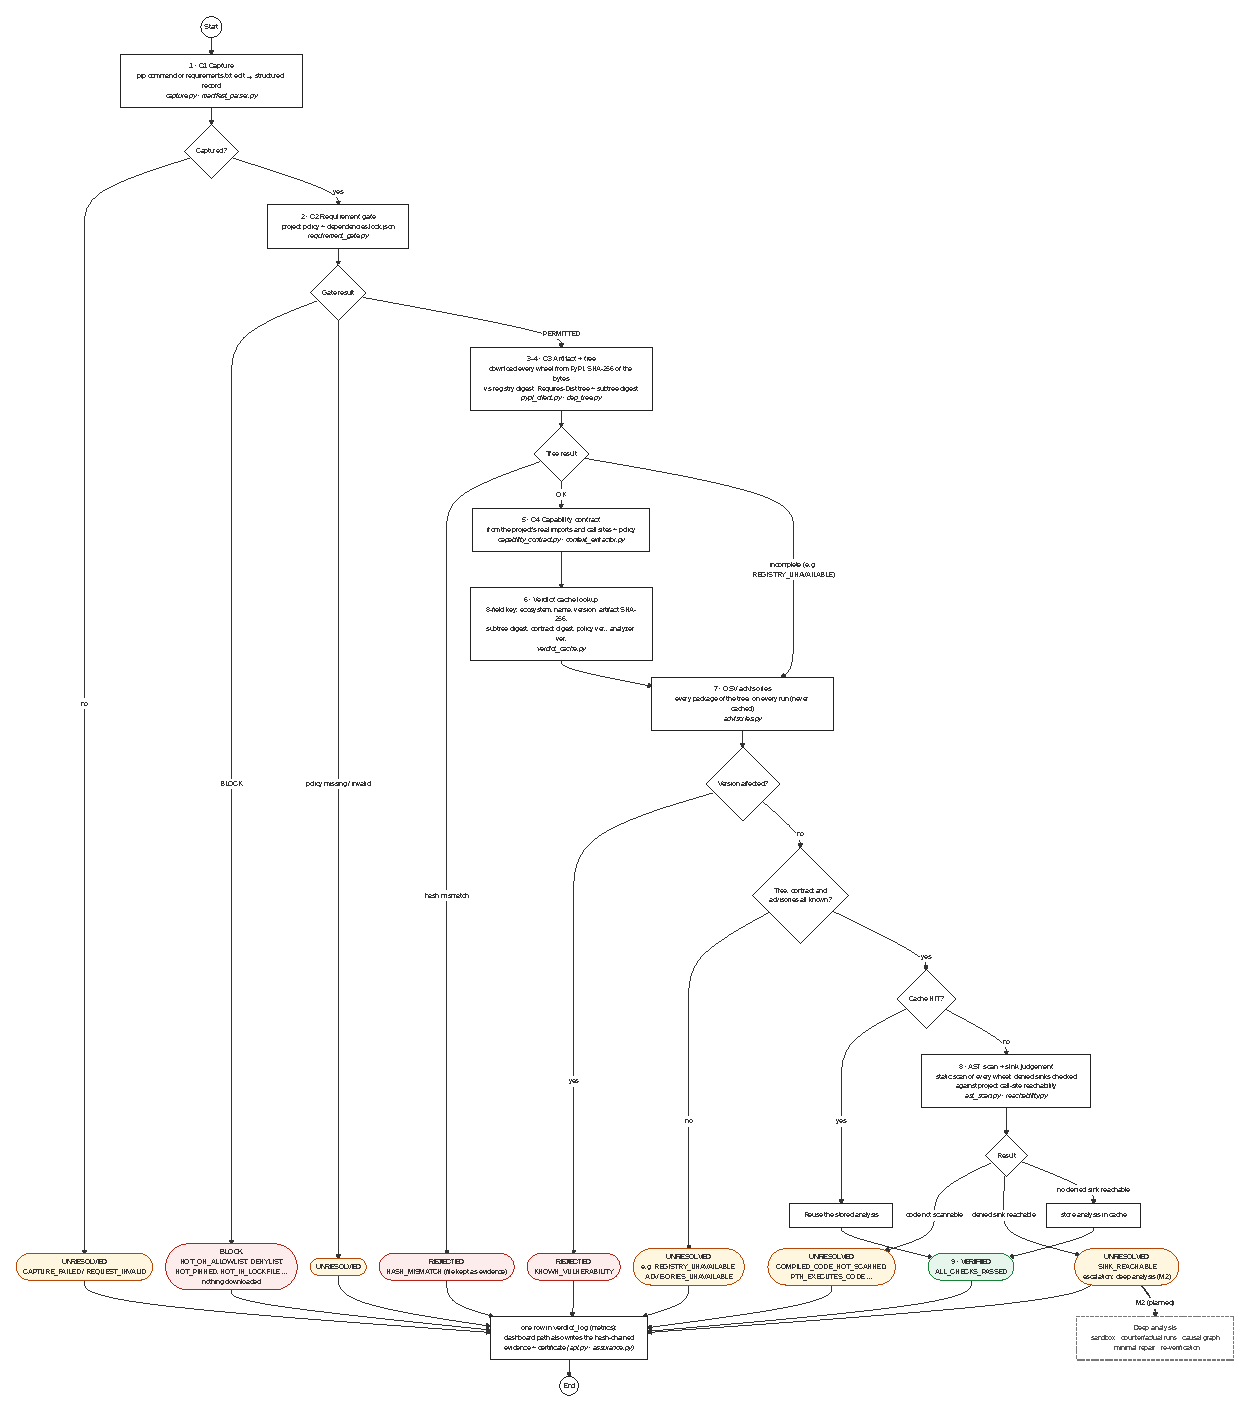
\includegraphics[height=0.88\textheight]{figures/diagrams/cavr-activity.pdf}
\caption{Activity diagram of the CAVR fast gate, \texttt{verify\_request} in \texttt{backend/cavr/pipeline.py}. Numbers follow the stage order in the code; the dashed element is planned (M2).}
\label{fig:cavr-activity}
\end{figure}

Figure~\ref{fig:cavr-activity} follows \texttt{verify\_request} stage by stage. The request is captured as a structured record (1) and checked by the requirement gate against the project policy and the lockfile (2); a request that is not permitted ends as \texttt{BLOCK} before anything is downloaded. Every wheel of the dependency tree is then downloaded from PyPI and its SHA-256 compared with the registry digest, and the tree and its subtree digest are built from the real \texttt{Requires-Dist} metadata (3--4); a mismatch is \texttt{REJECTED}. The capability contract is inferred from the project's own imports and call sites (5); only then can the 8-field cache key be formed and looked up (6), because it contains the contract digest. OSV is asked for every package of the tree on every run, also on a cache hit (7): an affected version is \texttt{REJECTED}, and any unknown input (registry, contract or advisories) is \texttt{UNRESOLVED}. On a cache miss the wheels are scanned statically and every denied sink is judged against the project's call-site reachability (8). A reachable denied sink is not treated as proven malicious: the verdict is \texttt{UNRESOLVED} with an escalation to M2 deep analysis. Only a complete analysis is stored in the cache. Every verdict writes one row to the verdict log; requests made from the dashboard also write the hash-chained evidence and the certificate.

\begin{figure}[htbp]
\centering
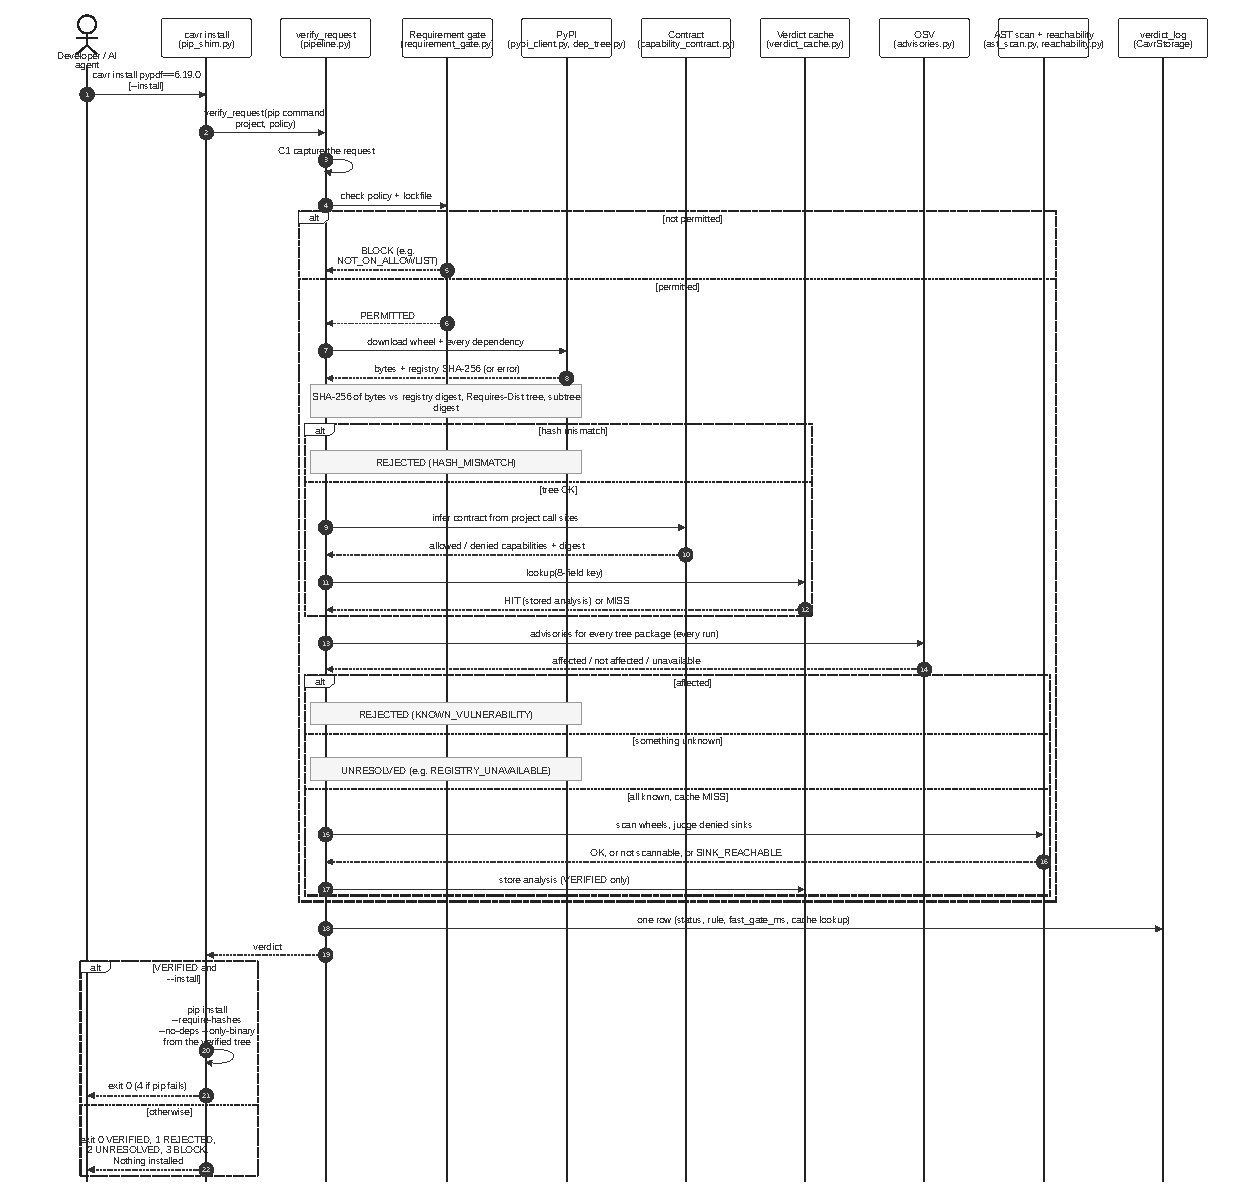
\includegraphics[width=\textwidth]{figures/diagrams/cavr-sequence.pdf}
\caption{Sequence of a \texttt{cavr install} request (\texttt{pip\_shim.py}) through \texttt{verify\_request} and its collaborators, with the wrapper's exit codes.}
\label{fig:cavr-sequence}
\end{figure}

Figure~\ref{fig:cavr-sequence} shows the same pipeline as messages between components. The wrapper never passes the user's arguments to pip; it only calls \texttt{verify\_request} and prints the verdict (exit code 0 \texttt{VERIFIED}, 1 \texttt{REJECTED}, 2 \texttt{UNRESOLVED}, 3 \texttt{BLOCK}). Only with \texttt{--install} and a \texttt{VERIFIED} verdict does it write a requirements file of the verified tree with \texttt{--hash=sha256} pins and run pip with \texttt{--require-hashes --no-deps --only-binary :all:}, so pip cannot install a different file, an unverified dependency or an sdist; a pip failure gives exit code 4.

\begin{figure}[htbp]
\centering
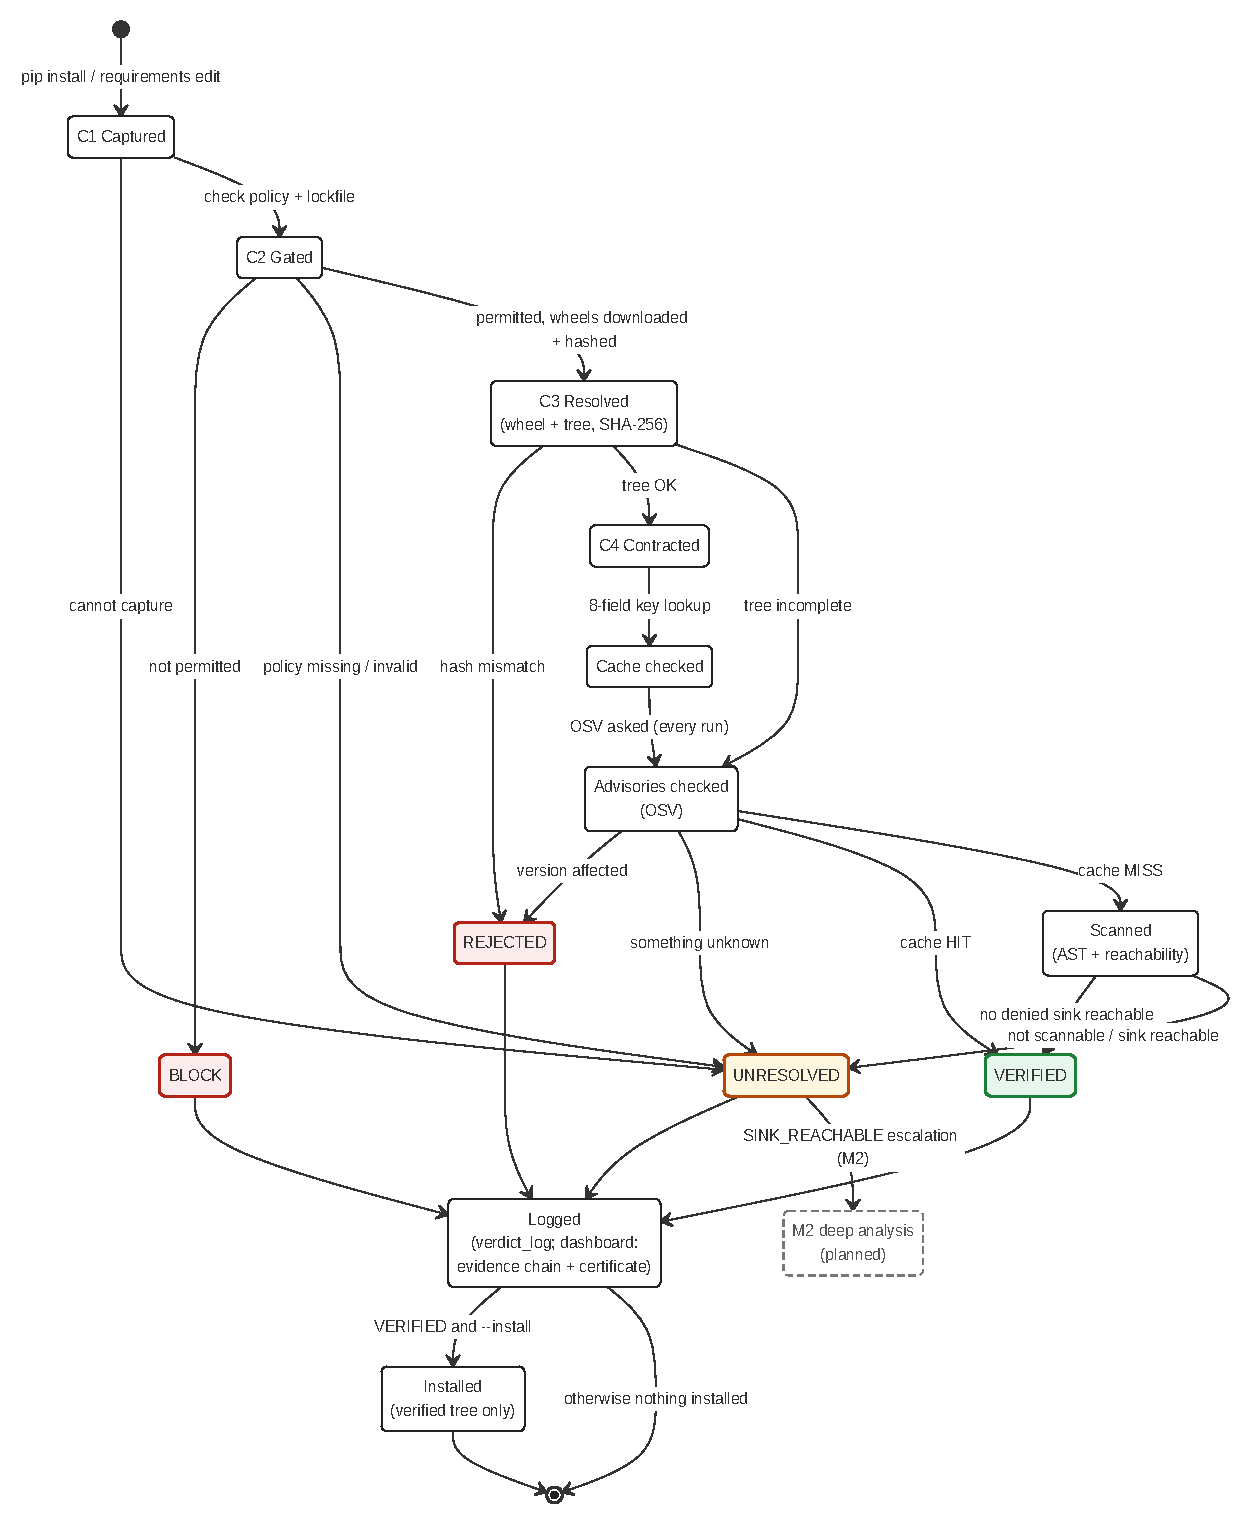
\includegraphics[width=0.85\textwidth]{figures/diagrams/cavr-state.pdf}
\caption{Lifecycle of a CAVR request. All four verdicts are logged; only a \texttt{VERIFIED} request with \texttt{--install} is installed.}
\label{fig:cavr-state}
\end{figure}

Figure~\ref{fig:cavr-state} shows the states of one request. \texttt{REJECTED} is reached only with positive evidence of a problem (a hash mismatch or an OSV advisory); every gap in the evidence leads to \texttt{UNRESOLVED}, which is never treated as a pass. \texttt{UNRESOLVED} with \texttt{SINK\_REACHABLE} is the state that M2 deep analysis will take over.
